\documentclass[a4paper,png]{article}
\usepackage[utf8]{inputenc}
\usepackage[L7x]{fontenc}
\usepackage[lithuanian]{babel}
\usepackage{lmodern}
\usepackage{amsmath,amssymb}
\usepackage[top=2cm, bottom=2cm, left=1.4cm, right=1.4cm, footskip=1cm, a4paper]{geometry}
\usepackage{indentfirst}
\usepackage{graphicx}
\usepackage{mdframed}
\usepackage{xcolor}
\usepackage{hyperref}
\usepackage{bm}
\usepackage{cancel}
\usepackage{framed}
\usepackage{indentfirst}

\begin{document}
Paprastų tiesinių nelygybių sprendimo eiga mažai skiriasi nuo tiesinių lygčių sprendimo: 

$(x+2)(x+1) < x(x+5) $

$ x^2+3x+2 < x^2+5x$

$\cancel{x^2}+3x+2 < \cancel{x^2}+5x $

$ 3x+2 < 5x $

$ 3x-5x+2 < 0 $

$ 3x-5x <-2 $

$ -2x <-2 $

\fbox{$x > 1$} Nepražiopsokite, kada pasikeičia nelygybės ženklas!

Šios nelygybės sprendime specifiniai metodai nebuvo reikalingi. Sudėtingesnių nelygybių atveju rekomenduoju naudoti intervalų metodą.
\section*{Reiškinių $(x+2)(x-3)(x-5)$ ir $(x+6)(x+1)(x-4)$ įgyjami ženklai}
Čia yra pateikiama pora įžanginių intervalų metodo prasmę iliustruojančių pavyzdžių, paimtų iš 1990 m. išleisto rusiško vadovėlio ALGEBRA (1999m. išverstas į lietuvių kalbą). Siūlau atkreipti dėmesį į teiginį:

\begin{mdframed}[backgroundcolor=yellow!50!white]
Kai $x$ pereina taškus, kuriuose reiškinys įgyja nulinę reikšmę, tai keičiasi reiškinio ženklas.
\end{mdframed}

Pirmo pavyzdžio sprendime atsispindi paaiškinimas, kodėl šis teiginys galioja, o antro pavyzdžio sprendime parodyta, kaip šį teiginį pritaikyti.
\newline
\begin{minipage}[b]{0.49\textwidth}
\fbox{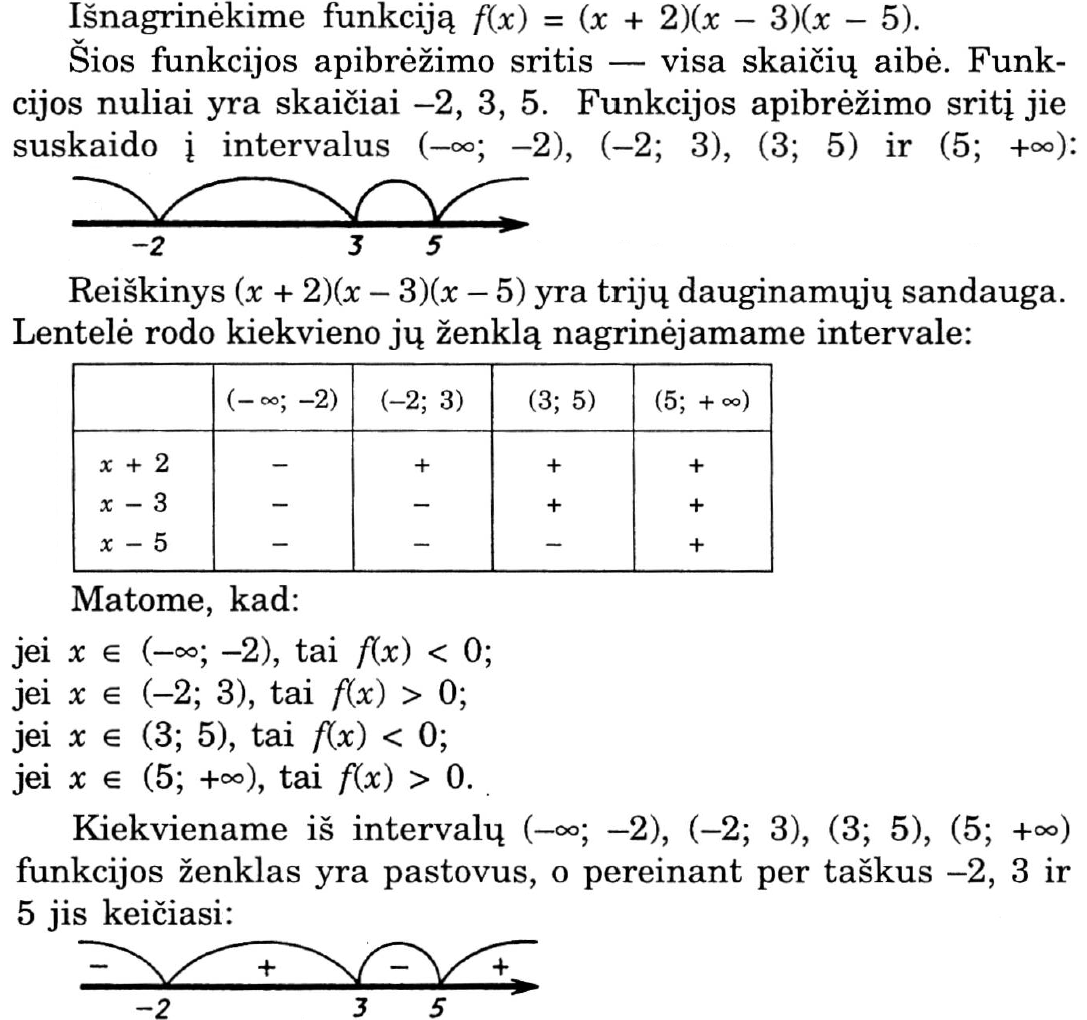
\includegraphics[width=\textwidth]{reiskzenklas.png}}
\end{minipage}
\hspace{\fill}
\begin{minipage}[b]{0.49\textwidth}
\fbox{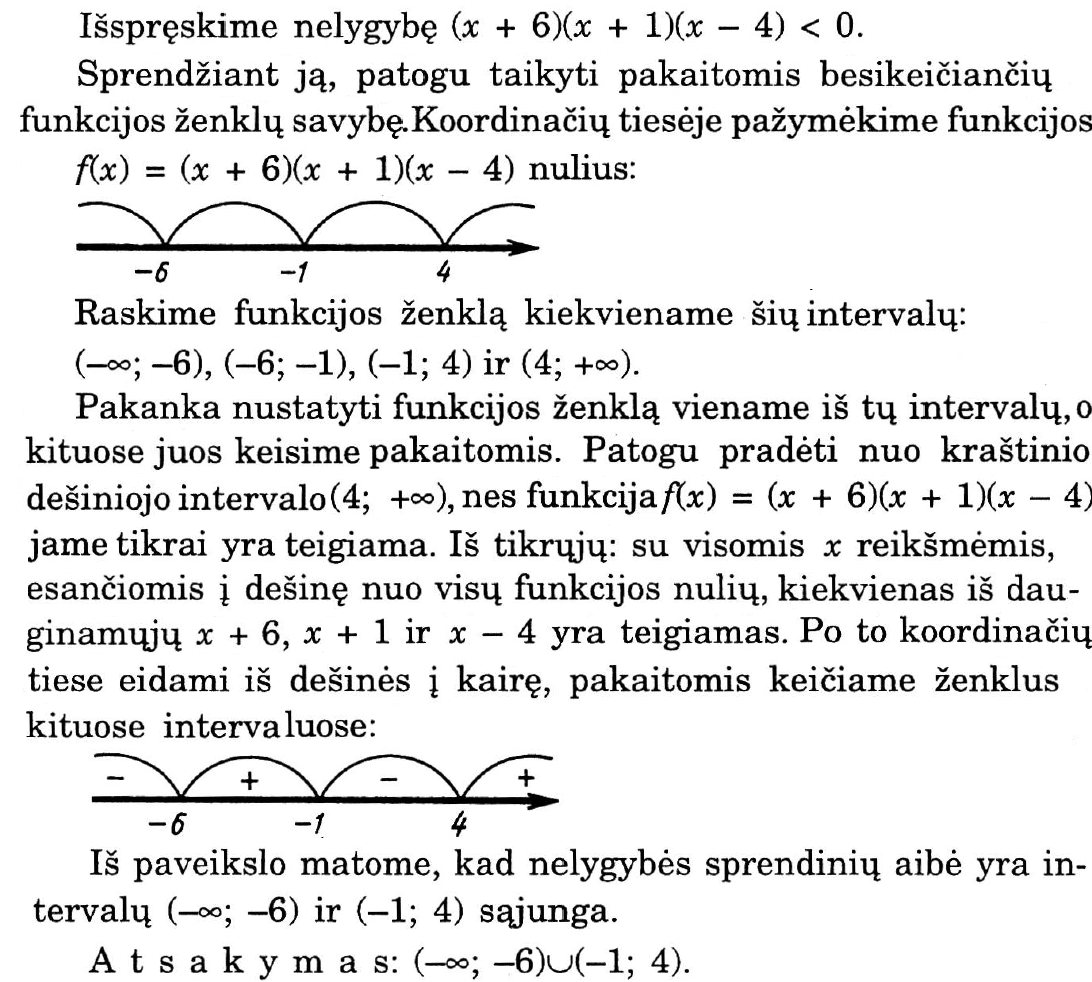
\includegraphics[width=\textwidth]{intpvz2.png}}
\end{minipage}
\newline
\newline
Abudu pavydžius galime apibendrinti:
\newline
\newline
\begin{minipage}[m]{0.49\textwidth}
\fbox{
\includegraphics[width=\textwidth]{intpvz3.png}}
\end{minipage}
\hspace{\fill}
\begin{minipage}[b]{0.49\textwidth}
\fbox{$\begin{array}{l}
\text{\phantom{xxx}Funkcijos $f(x)=(x-x_1)(x-x_2)\dots (x-x_n)$ reikšmės}
\\\text{išsidėsto vienu iš šių būdų:}
\\
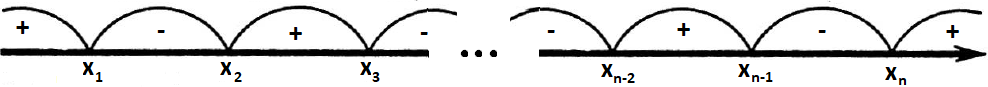
\includegraphics[width=0.9\textwidth]{longplusn.png}\\
\text{\phantom{xxx}arba}\\
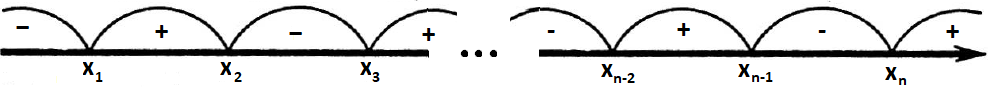
\includegraphics[width=0.9\textwidth]{longminusn.png}
\end{array}$}
\end{minipage}
\renewcommand\thesection{}
\section[]{Nelygybių suvedimas į vieną iš formų \small{$\begin{array}l(x-x_1)(x-x_2)\dots (x-x_n)>0 \\ (x-x_1)(x-x_2)\dots (x-x_n)<0\end{array}$}}
Šiame skyrelyje nelygybėms intervalo metodo netaikysime, tik nagrinėsime, kaip jas suvesti į formą, tinkamą taikyti intervalų metodą.
\subsection*{Paprasti pertvarkymai}
Remiantis vien intervalų metodu išsprendžiamos visos mokyklinės nelygybės, į kurias neįeina sudėtingesnės mokyklinės funkcijos (jomis laikome eksponentines ir trigonometrines funkcijas bei joms atvirkštines). Paprasčiausia spręsti nelygybes, į kurias įeina tik daugianariai arba iš jų sudarytos trupmenos. Tačiau intervalų metodas veiksmingas tik tuomet, kai nelygybė yra suvedama į vieną iš formų {\small{$\begin{array}l(x-x_1)(x-x_2)\dots (x-x_n)>0 \\ (x-x_1)(x-x_2)\dots (x-x_n)<0\end{array}$}}. Čia pateiksiu keletą tokio suvedimo pavydžių.
\begin{enumerate}
\item Suvesime nelygybę \fbox{$x(0,5-x)(x+4)<0$}. Pirmiausia iškelsime už skliaustų daugianario $0,5-x$ dauginamąjį -1. Gausime nelygybę $-x(x-0,5)(x+4)<0$. Iš čia \fbox{$x(x-0,5)(x+4)>0$}. (Čia į daugiklį $x$ galime žiūrėti kaip į daugiklį $x-0$)
\item Suvesime nelygybę \fbox{$(5x+1)(5-x)>0$}. Iškėlę už skliaustų pirmojo dvinario dauginamąjį $5$, o antrojo $-1$ gauname nelygybę $-5\left(x+\frac{1}{5}\right)(x-5)>0$. Dabar abi nelygybės formas padaliję iš $-5$ gauname tai, ką reikėjo:
\fbox{$\left(x+\frac{1}{5}\right)(x-5)<0$.}
\item Suvesime nelygybę \fbox{$\frac{7-x}{x+2}<0$}. Galima pastebėti, kad trupmenos $\frac{7-x}{x+2}$ ženklas sutampa su sandaugos $(7-x)(x+2)$ ženklu. Vadinasi nelygybė gali būti pakeista į $(7-x)(x+2)<0$, o šią nelygybę daugindami iš $-1$ pertvarkome į \fbox{$(x-7)(x+2)>0$}.
\end{enumerate}
\subsection*{Skaidymas dauginamaisiais (kvadratinėms nelygybėms)}
Dažnai egzamine intervalų metodu prireikia spręsti kvadratines nelygybes. Šiuo atveju nelygybės gali būti pertvarkomos, kad dešinėje pusėje gautume $0$, o kairėje pusėje gautume kvadratinį reiškinį. Dalis tokių reiškinių negali įgyti nulinės reikšmės, vadinasi negali būti išskaidyti dauginamaisiais ir sprendžiami intervalų metodu. Pavyzdžiui:
\begin{itemize}
\item $3x^2+5$ yra teigiamas su visais $x$, nes pirmas dėmuo neneigiamas, o antras dėmuo teigiamas su visais $x$. 
\item Kvadratiniai trinariai, kurių diskriminantas neigiamas, įgyja tik vienodo ženklo reikšmes.
\end{itemize} 
Visais šiais atvejais nelygybė arba sprendinių neturės, arba galios su visais $x$. Apibendrinę pastebėjimus gauname:

\begin{mdframed}[backgroundcolor=yellow!50!white]
Kvadratiniai trinariai $ax^2+bx+c$ su neigiamu diskriminantu yra neišskaidomi ir turi vienodą ženklą su visais $x$
\end{mdframed}

Likusi kvadratinių reiškinių dalis gali įgyti nulines reikšmes, vadinasi gali būti suvesti į formą $a(x-x_1)(x-x_2)$ ir sprendžiami intervalų metodu. Kvadratinius trinarius skaidyti sudėtinga. Tokiu atveju pasinaudojame faktu:

\begin{mdframed}[backgroundcolor=yellow!50!white]
Kvadratinio trinario $ax^2+bx+c$ skaidinys yra $a(x-x_1)(x-x_2)$, kur $x_1$ ir $x_2$ yra šio reiškinio šaknys.
\end{mdframed}

Štai keletas kvadratinių nelygybių suvedimo į tinkamą formą pavyzdžių:
\begin{enumerate}
\item Suvesime nelygybę \fbox{$x^2+3x \leq 0$}. Dešinėje pusėje turime $0$, todėl kairę pusę galime išskaidyti. Skaidymas paprastas: \fbox{$x(x+3) \leq 0$}.
\item Suvesime nelygybę \fbox{$x^2 \leq 9$}. Pertvarkome, kad dešinėje pusėje būtų $0$ ir gauname nelygybę $x^2 - 9\leq 0$ . Dešinę pusę išskaidome pagal kvadratų skirtumo formulę: \fbox{$(x+3)(x-3) \leq 0$}.
\item Suvesime nelygybę \fbox{$x^2-3x>-2$}. Pertvarkome, kad dešinėje pusėje būtų $0$ ir gauname nelygybę
 $x^2-3x+2>0$. Dabar kairę pusę galime išskaidyti. Kvadratinės lygties $x^2-3x+2 = 0$ sprendiniai yra $x_1=1\text{ ir } x_2=2$. Pagal formulę $ax^2+bx+c = a(x-x_1)(x-x_2)$ nelygybę galime pertvarkyti į \fbox{$(x-1)(x-2)>0$}.
\item Suvesime nelygybę \fbox{$x^2+4<3x$}. Pertvarkome, kad dešinėje pusėje būtų $0$ ir gauname nelygybę
 $x^2-3x+4<0$. Trinario $x^2-3x+4$ diskriminantas yra neigiamas, todėl jis neturi skaidinio ir nelygybė negali būti suvesta į reikiamą formą. Šis trinaris įgyja tik teigiamas reikšmes, vadinasi \fbox{$x \in \emptyset$}.
\end{enumerate}
\section{Suvestų į tinkamą formą nelygybių sprendimas}
Ankstesniame skyriuje aptarėme techninę dalį: kaip atlikti nelygybės pertvarkymus norint ją suvesti į tinkamą formą intervalų metodui taikyti. Pats intervalų metodų taikymas yra lengvoji sprendimo dalis. Šiame skyriuje sudarysime lentelę, parodančią visus pagrindinius kiekvienos nelygybės sprendimo etapus. Prieš pateikiant sprendimus - dar viena svarbi pastaba:
\begin{mdframed}[backgroundcolor=yellow!50!white]
\begin{itemize}
\item Perėjimo taškai skaičių ašyje žymimi kaip pilnaviduriai, jei jie tenkina nelygybę (atveju $\le$ arba $\ge$). Jie į sprendinį įtraukiami.
\item Perėjimo taškai skaičių ašyje žymimi kaip tuščiaviduriai, jei jie nelygybės netenkina (atveju $<$ arba $>$). Jie į sprendinį neįtraukiami.
\end{itemize}
\end{mdframed}
\noindent
\begin{tabular}{|l|l|l|l|l|}
\hline
Nelygybė & Suvedimas & \small{$\begin{array}{c}\text{Perėjimo} \\ \text{taškai} \end{array}$}& Brėžinys & Atsakymas\\\hline
$x(0,5-x)(x+4)<0$ & $x(x-0,5)(x+4)>0$ & 0, 0,5 ir -4 & \raisebox{-0.6\height}{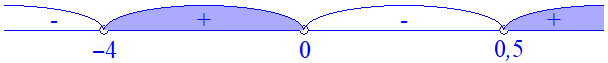
\includegraphics[width=0.25\textwidth]{interval5.png}} &$x\in(-4;0)\bigcup (0,5;+\infty)$\\\hline
$(5x+1)(5-x)>0$ & $\left(x+\frac{1}{5}\right)(x-5)<0$ & $-\frac{1}{5}$ ir 5 & \raisebox{-0.5\height}{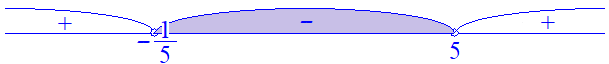
\includegraphics[width=0.25\textwidth]{interval6.png}} &$x\in\left(-\frac{1}{5};5\right)$\\\hline
$\frac{7-x}{x+2}<0$ & $(x-7)(x+2)>0$ & 7 ir $-2$ & \raisebox{-0.6\height}{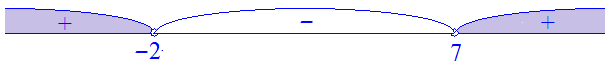
\includegraphics[width=0.25\textwidth]{interval3.png}} &$x \in(-\infty;-2)\bigcup(7;+\infty)$\\\hline
$x^2\geq 9$ & $(x+3)(x-3) \geq 0$ & $-3$ ir 3 & \raisebox{-0.6\height}{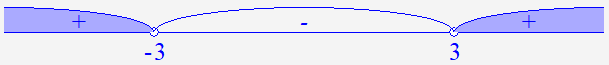
\includegraphics[width=0.25\textwidth]{interval4.png}} & $x \in(-\infty;-3]\bigcup[3;+\infty)$\\\hline
$x^2+3x \leq 0$ & $x(x+3) \leq 0$ & 0 ir $-3$ & \raisebox{-0.6\height}{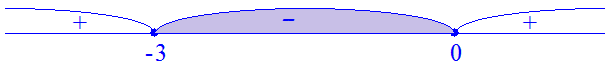
\includegraphics[width=0.25\textwidth]{interval1.png}} &$x \in[-3;0]$\\\hline
$x^2-3x>-2$ & $(x-1)(x-2)>0$ & 1 ir 2 & \raisebox{-0.6\height}{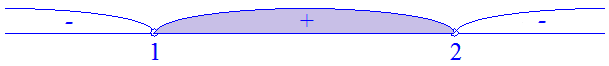
\includegraphics[width=0.25\textwidth]{interval2.png}} &$x \in(-\infty;1)\bigcup(2;+\infty)$\\\hline
$x^2+4<3x$ & nesuvedama & nėra & $\begin{array}{l}\text{trinaris $x^2-3x+4$ su visais}\\\text{$x$ bus teigiamas}\end{array}$ &$x\in \emptyset$ \\\hline
$x^2+9<0$ & nesuvedama & nėra & $\begin{array}{l}\text{reiškinys $x^2+9$ su visais $x$}\\\text{neįgyja neigiamų reikšmių}\end{array}$ &$x\in \emptyset$ \\\hline
\end{tabular}
Pagal brėžinius galima pastebėti, jog kiekvieno kvadratinio trinario reikšmės didinant kintamąjį visuomet išsidėsto tvarka +, -, +. Kodėl taip yra? Atsakymo ieškokite tarp pirmo skyriaus gale pateiktų brėžinių.
\section*{Sudėtingesni atvejai}
Čia pateiksime keletą sudėtingesnių atvejų, kurių sprendimo intervalų metodu eiga yra kiek kitokia, nei įprasta.
\subsection*{Atvejai, kuomet reikia atsižvelgti į apibrėžimo sritį}
Čia pateiksiu pavyzdį iš vadovėlio \textit{Matematika. Bendrasis kursas XI klasei (2005m.)}:

\fbox{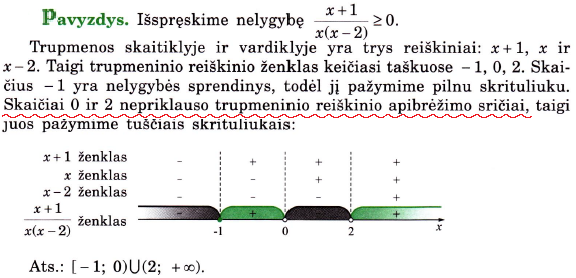
\includegraphics[width=0.5\textwidth]{apsritis.png}}

Priminsime, kad:
\begin{mdframed}[backgroundcolor=yellow!50!white]
reiškinio apibrėžimo sritis - tai visos $x$ reikšmės, su kuriomis jis turi prasmę.
\end{mdframed}
Daugumos mokyklinių reiškinių apibrėžimo sritis yra visi realieji skaičiai. Likusiais atvejais patartina įsiminti sąlygas, su kuriomis reiškiniai yra apibrėžti:

\noindent
\begin{mdframed}[backgroundcolor=yellow!50!white]
\begin{tabular}{|l|l|l|l|}
\hline
Reiškinys & Apibrėžimo sritis & Apribojimas & Apribojimas reiškiniui bendresniu atveju\\
\hline
$f(x)=\frac{1}{x}$ & $(-\infty; 0)\bigcup (0;+\infty)$ & $x\neq 0$ & Vardiklis įgyja tik nenulines reikšmės \\
\hline
$f(x)=\sqrt{x}$ & $[0;+\infty)$ & $x\ge 0$ & Lyginio laipsnio šaknies pošaknis įgyja tik neneigiamas reikšmes\\
\hline
$\log_{a}x$ & $(0;+\infty)$ & $x>0$ & Pologaritminis reiškinys įgyja tik teigiamas reikšmes\\
\hline
\end{tabular}
\end{mdframed}

Kitas pavydys iš 2015 metų VBE, kuriame pilnas nelygybės $\log_{0,2}(4x-5)+\log_{0,2}(2x+3)\ge \log_{0,2}13$ sprendimas buvo įvertintas net 7 taškais (iš 60 egzamine galimų). Šis egzamino uždavinys susidėjo iš 2 dalių:
\newline
\newline
\begin{minipage}[b]{0.49\textwidth}
\begin{itemize}
\item Nustatyti reiškinio $\log_{0,2}(4x-5)+\log_{0,2}(2x+3)$ apibrėžimo sritį (2 taškai).
\item Išspręsti pateiktą nelygybę (5 taškai).
\end{itemize}
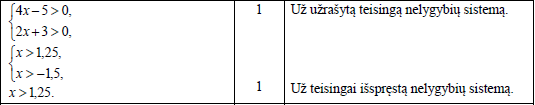
\includegraphics[width=\textwidth]{egznelyg_apibr.png}
\end{minipage}
\hspace{\fill}
\begin{minipage}[t]{0.49\textwidth}
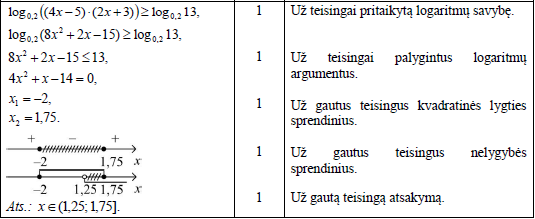
\includegraphics[width=\textwidth]{egznelyg.png}
\end{minipage}
\newline\par
Šiame VBE vertinimo instrukcijose pateiktame sprendime ne visur išlaikomas aiškumas. Nelygybės $8x^2+2x-15\le 13$ pertvarkymas į lygtį $4x^2+x-14=0$ įprastai nėra leistinas, kas kelia abejonių dėl šio sprendimo aiškumo. Apibrėžimo srities nustatymo nenagrinėsime, tik prisiminsime, jog nelygybė apibrėžta, kai \fbox{$x>1,25$}. Panašiai, kaip ir ankstesnių pratimų atveju galima užpildyti nelygybės $\log_{0,2}(4x-5)+\log_{0,2}(2x+3)\le \log_{0,2}13$ sprendimo etapus parodančią lentelę:

\begin{tabular}{|l|l|l|l|}
\hline
Suvedimas & \small{$\begin{array}{c}\text{Perėjimo} \\ \text{taškai} \end{array}$}& Brėžinys (pagal VBE) & Atsakymas\\\hline
$4(x-1,75)(x+2)\le 0$ & 1,75 ir -2 & \raisebox{-0.6\height}{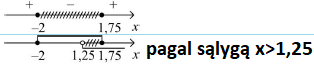
\includegraphics[width=0.25\textwidth]{intervalvbe.png}} &$x\in(1,25;1,75]$\\\hline
\end{tabular}
\newline\par
Nelygybės suvedimas į tinkamą formą buvo sudėtingiausia šio uždavinio dalis. Remdamiesi logaritmų savybėmis nelygybę galime pertvarkyti į $8x^2+2x-15\le 13$, o vėliau į $4x^2+x-14\le 0$. Kairės pusės kvadratinio trinario skaidinys yra $4(x-x_1)(x-x_2)$, kur $x_1$, $x_2$ yra šio trinario šaknys. Jas gauname spręsdami lygtį $4x^2+x-14=0$. Jos lygios 1,75 ir $-2$, todėl nelygybė suvedama į \fbox{$4(x-1,75)(x+2)\le 0$}.
\subsection*{Atvejai, kuomet reiškinyje yra pakartotinių daugiklių}
Reiškinį $x^2(x+1)$ galima užrašyti kaip sandaugą $x\cdot x\cdot (x+1)$. Matome, kad sandaugoje yra pakartotinis daugiklis $x$. Jo laipsnis yra 2. Nors daugiklių yra trys, tačiau reiškinio ženklo perėjimo taškai gali būti tik 0 ir $-1$. 
\begin{mdframed}[backgroundcolor=yellow!50!white]
Jei daugiklis pakartotinis ir lyginio laipsnio, tuomet jį atitinkantis perėjimo taškas nekeičia ženklo.
\end{mdframed}
Pailiustruosime šią taisyklę 2018metų VBE 8 uždavinio (1 tšk) sprendimu.

\begin{tabular}{|l|l|l|l|}
\hline
Nelygybė & \small{$\begin{array}{c}\text{Perėjimo} \\ \text{taškai} \end{array}$}& Brėžinys & Atsakymas\\\hline
$x^2(x+1)>0$ & 0 ir -1 & \raisebox{-0.6\height}{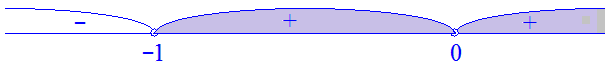
\includegraphics[width=0.25\textwidth]{interval2018.png}} &$x\in(-1;0)\bigcup (0;+\infty)$\\\hline
\end{tabular}
\section*{Visi uždaviniai iš 2010 - 2018 VBE, kuriuos sprendžiant galima remtis intervalų metodu}
Žvaigždute pažymėti uždaviniai reikalauja žinių iš kitų sričių arba gilesnio supratimo.
\begin{enumerate}
\item (\textit{\textbf{VBE 2018, 19.2}}) Raskite didžiausią natūralųjį skaičių $n$, tenkinantį nelygybę $\frac{n(n+1)}{2}<1009$ [1 tšk.]
\item (\textit{\textbf{VBE 2018, 8}}) Išspręskite nelygybę $x^2(x+1)$ [1 tšk.]
\item (\textit{\textbf{VBE 2018, 15.2}}) Išspręskite nelygybę $x(x-1)<20$ [0.5 tšk.]
\item (\textit{\textbf{VBE 2016, 9}}) Išspręskite nelygybę $x(x-1)\le 20$ [1 tšk.]
\item (\textit{\textbf{VBE 2016, 19.3}}) Išspręskite nelygybę $\frac{x}{(x+2)(x-1)}\ge 0$ [2 tšk.]
\item (\textit{\textbf{VBE 2015, 20.2}}) Išspręskite nelygybę $(2x+3)(4x-5)\le 13$ [2,5 tšk.]
\item (\textit{\textbf{VBE 2014band., 4}}) Išspręskite nelygybę $x^2<x$
\item (\textit{\textbf{VBE 2014band., 28*}}) Nustatykite didžiausią reiškinio $\frac{1}{2}-t^2+t$ reikšmę, kai $t\in [0;1]$
\item (\textit{\textbf{VBE 2014, 19}}) Išspręskite nelygybę $5-x^2\le 4$ [1tšk.]
\item (\textit{\textbf{VBE 2014, 25.1*}}) Nustatykite reiškinio $\log_{\frac{1}{2}} (x^2-7x+10)$ apibrežimo sritį [2tšk.]
\item (\textit{\textbf{VBE 2014, 25.2*}}) Raskite visas $x$ reikšmes, su kuriomis funkcijos $f(x)=\log_{\frac{1}{2}} (x^2-7x+10)$ reikšmės yra ne mažesnės už -2. [3tšk.]
\item (\textit{\textbf{VBE 2013 ir 2011, 5}}) Išspręskite nelygybę $x^2>(x-1)^2$ [1tšk.]
\item (\textit{\textbf{VBE 2010, 18*}}) Nustatykite funkcijos $f(x)=\frac{1}{4}(x-2)^2(x+1)$ didėjimo ir mažėjimo intervalus , kai duota, jog $f'(x)=\frac{3}{4}x^2-\frac{3}{2}$ [2tšk.]
\end{enumerate}
\section*{Pastabos}
Nelygybes spręsti galima ir remiantis kitokiais metodais: grafiniu ir algebriniu, tačiau intervalų metodą laikome paprasčiausiu.
\end{document}